% ju 04-Nov-20
\documentclass[a4paper,12pt]{scrartcl}
% letztes Update: 1-Jun-20

% Eingabe der Metadaten

%-------Daten des Autors--------------------------
\newcommand{\autor}{Jan Unger}
\newcommand{\ort}{Wuppertal}
\newcommand{\website}{https://bw-ju.de/}

%-------Titel und Untertitel-----------------------
\newcommand{\titel}{Notizen-TeX-Web}% THEMA 
\newcommand{\untertitel}{Projekt}% keinen Untertitel 
\newcommand{\typ}{\LaTeX}

%-------Datum: Jahr/Monat/Tag ---------------------
\newcommand{\version}{\today}% DATUM:  \date{2020/06/30}  o. \today

%-deutsche Schlagwoerter(bitte getrennt durch Kommata auflisten)
\newcommand{\schlagwoerter}{PDF, Latex, Markdown, Pandoc, Git, Texlive}



%% anpassen
\usepackage{praeambel-artikel}% Pakete
% Literatur laden
\bibliography{content/literatur}      %% anpassen
\bibliography{content/literatur-kfz}  %% anpassen
\bibliography{content/literatur-sport}%% anpassen
%% anpassen
\title{Spickzettel-Markdown}
\author{\autor}
\date{\today}
%\date{2020/08/01}%% anpassen
%\date{1-Aug-20}
%
\begin{document}
	%% anpassen
	%\maketitle
	%\tableofcontents  
	%\listoffigures 
	%\listoftables 
	%\lstlistoflistings

	%% anpassen	
	%\begin{abstract}
	%	Zusammenfassung
	%\end{abstract}

	%% anpassen
	%-------------------------------------------------
	%
		% letztes Update: 10-Aug-20
\section{Schreiben in Markdown}\label{schreiben-in-markdown}

\begin{enumerate}
\item
  Markdown
\item
  Textauszeichnung -- Was ist wichtig?, Tabellen, Bilder, Quellcode,
  Literatur, Links
\item
  Rechtschreibprüfung \footnote{\url{https://languagetoolplus.com/?pk-campaign=addon2-popup-logo}}
\item
  Literatur \footnote{\url{https://www.zotero.org/user/login}}
\end{enumerate}

\section{Markdown -- Latex -- PDF
erstellen}\label{markdown-latex-pdf-erstellen}

\begin{enumerate}
\item
  Markdown > Latex: \verb|$ projekt.sh|
  Script (pandoc)
\item
  Hand-Kopie: \verb|tex\_pandoc/ tex/|
\item
  Referenzen: Links prüfen

  \begin{itemize}
  \item
    Bild %vgl.~(\autoref{fig:}). >
    \verb|(\\autoref\{fig:bild\}).|
  \item
    Tabelle %vgl.~(\autoref{tab:}). >
    \verb|(\\autoref\{tab:tabellen\}).|
  \item
    Kapitel %vgl.~(\autoref{}). >
    \verb|(\\autoref\{sec:zusammenfassung\}).|
  \item
    Code %vgl.~(\autoref{code:}). >
    \verb|(\\autoref\{code:hallowelt\})|.
  \end{itemize}
\item
  Latex > PDF: \verb|$ make| Makefile
  (latexmk)
\end{enumerate}

\section{Quellen}\label{quellen}

Quelle: ~\textcite{monk:2016:action}

Quelle: ~\textcite{homofaciens:2018:projekt}

Quelle: ~\textcite{kofler:2018:hacking}

\lstset{language=C}% C, TeX, Bash, Python 
\begin{lstlisting}[
	%caption={}, label={code:}%% anpassen
]
Quelle: [@monk:2016:action]
Quelle: [@homofaciens:2018:projekt]
Quelle: [@kofler:2018:hacking]
\end{lstlisting}

\section{Listen}\label{listen}

\textbf{ungeordnete Liste}

\begin{itemize}
\item
  a
\item
  b

  \begin{itemize}
  \item
    bb
  \end{itemize}
\item
  c
\end{itemize}

\lstset{language=C}% C, TeX, Bash, Python 
\begin{lstlisting}[
	%caption={}, label={code:}%% anpassen
]
- a
- b
    - bb
- c
\end{lstlisting}

\textbf{Sortierte Liste}

\begin{enumerate}
\item
  eins
\item
  zwei
\item
  drei
\end{enumerate}

\lstset{language=C}% C, TeX, Bash, Python 
\begin{lstlisting}[
	%caption={}, label={code:}%% anpassen
]
1. eins
2. zwei
3. drei
\end{lstlisting}

\textbf{Sortierte Liste}

\begin{enumerate}
\def\labelenumi{\alph{enumi})}
\item
  a
\item
  b
\item
  c
\end{enumerate}

\lstset{language=C}% C, TeX, Bash, Python 
\begin{lstlisting}[
	%caption={}, label={code:}%% anpassen
]
a) a
b) b
c) c
\end{lstlisting}

\section{Anführungszeichen}\label{anfuehrungszeichen}

>>Anführungszeichen<<

\lstset{language=C}% C, TeX, Bash, Python 
\begin{lstlisting}[
	%caption={}, label={code:}%% anpassen
]
"Anführungszeichen" 
\end{lstlisting}

\section{Grafik -- Abbildung}\label{grafik-abbildung}

Grafiken-Bsp vgl.~(\autoref{fig:Grafiken-Bsp}).

\begin{figure}[!hb]% hier: !hb
\centering

\includegraphics[width=0.3\textwidth]{Grafiken/logo.eps}
\caption{Grafiken-Bsp}
\label{fig:Grafiken-Bsp}%% anpassen
\end{figure}

\lstset{language=C}% C, TeX, Bash, Python 
\begin{lstlisting}[
	%caption={}, label={code:}%% anpassen
]
![Grafiken-Bsp](Grafiken/logo.eps){width=30%}
\end{lstlisting}

Abbildung-Bsp vgl.~(\autoref{fig:Abbildung-Bsp}).

\begin{figure}[!hb]% hier: !hb
\centering
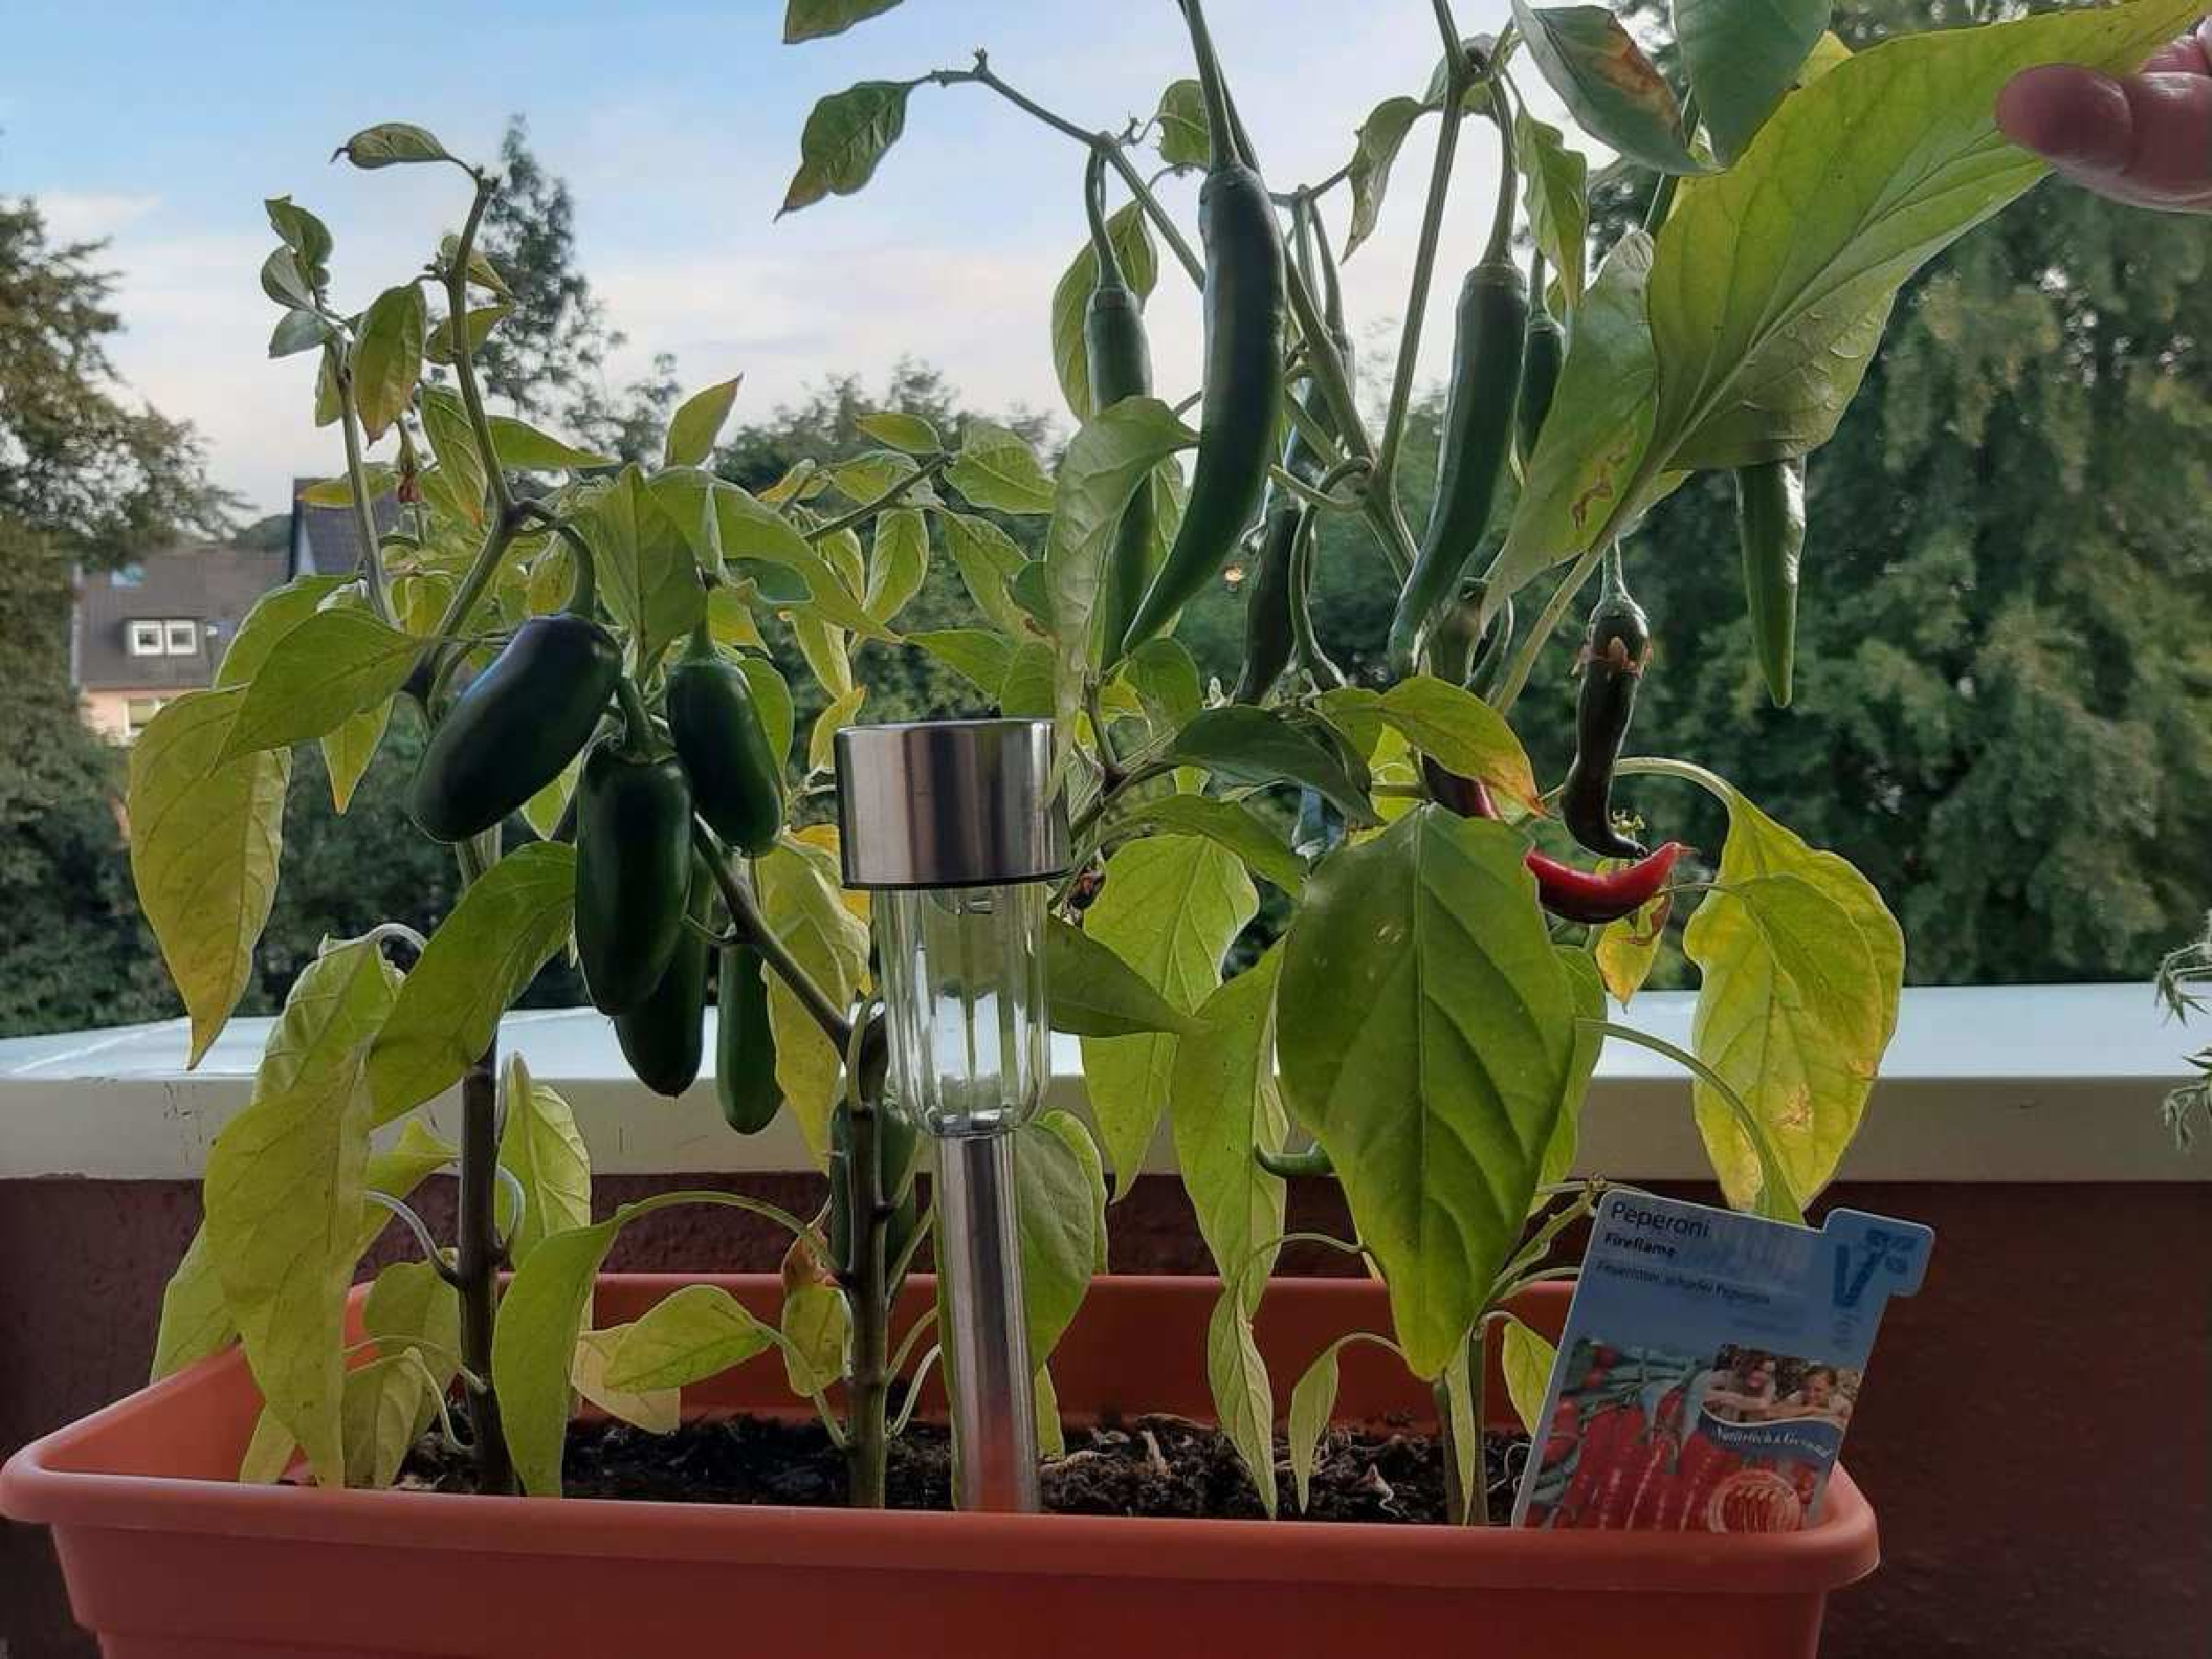
\includegraphics[width=0.6\textwidth]{images/Chili-1.pdf}
\caption{Abbildung-Bsp}
\label{fig:Abbildung-Bsp}%% anpassen
\end{figure}

\lstset{language=C}% C, TeX, Bash, Python 
\begin{lstlisting}[
	%caption={}, label={code:}%% anpassen
]
![Abbildung-Bsp](images/Chili-1.pdf){width=60%}
\end{lstlisting}

\section{Tabelle}\label{tabelle}

Tabelle-Bsp vgl.~(\autoref{tab:Tabelle-Bsp}).

\begin{table}[!ht]% hier: !ht 
\centering 
	\caption{Tabelle-Bsp} \label{tab:Tabelle-Bsp}%% anpassen 
\begin{tabular}{@{}rll@{}}
\toprule
\textbf{Nr.} & \textbf{Begriffe} & \textbf{Erklärung}\\
\midrule
1 & a1 & a2\\
2 & b1 & b2\\
3 & c1 & c2\\
4 & a1 & a2\\
\bottomrule
\end{tabular} 
\end{table}

\lstset{language=C}% C, TeX, Bash, Python 
\begin{lstlisting}[
	%caption={}, label={code:}%% anpassen
]
|**Nr.**|**Begriffe**|**Erklärung**|
|--:|:-----|:----|
| 1     | a1         | a2          
| 2     | b1         | b2          
| 3     | c1         | c2          
| 4     | a1         | a2          
\end{lstlisting}

\section{Mathe}\label{mathe}

$[ V ] = [ \Omega ] \cdot [ A ]$ o. $U = R \cdot I$ o.
$R = \frac{U}{I}$

\lstset{language=C}% C, TeX, Bash, Python 
\begin{lstlisting}[
	%caption={}, label={code:}%% anpassen
]
$[ V ] = [ \Omega ] \cdot [ A ]$ o. $U = R \cdot I$ o. $R = \frac{U}{I}$
\end{lstlisting}

$5~cm$, $a \cdot b$, $\cdots$, $\Omega$

$100^\circ\text{C}$

$80~\%$

\lstset{language=C}% C, TeX, Bash, Python 
\begin{lstlisting}[
	%caption={}, label={code:}%% anpassen
]
$5~cm$, $a \cdot b$, $\cdots$, $\Omega$
$100^\circ\text{C}$  
// ACHTUNG: Prozentzeichen macht Probleme in HTML und Latex 
// Z.B. 80 %
$80~\%$ // in Latex
$80~%$  // in HTML
\end{lstlisting}

\textbf{Matheumgebung:}

\begin{align*}
    \sum_{i=1}^5 a_i = a_1 + a_2 + a_3 + a_4 + a_5
\end{align*}

\lstset{language=C}% C, TeX, Bash, Python 
\begin{lstlisting}[
	%caption={}, label={code:}%% anpassen
]
\begin{align*}
    \sum_{i=1}^5 a_i = a_1 + a_2 + a_3 + a_4 + a_5
\end{align*}
\end{lstlisting}

\section{Texthervorhebung}\label{texthervorhebung}

\textbf{Fett} oder \emph{Kursiv}

\lstset{language=C}% C, TeX, Bash, Python 
\begin{lstlisting}[
	%caption={}, label={code:}%% anpassen
]
**Fett** oder *Kursiv*
\end{lstlisting}

\section{Code}\label{code}

HalloWelt vgl.~(\autoref{code:HalloWelt}).

\lstset{language=C}% C, TeX, Bash, Python 
\begin{lstlisting}[
	caption={HalloWelt}, label={code:HalloWelt}%% anpassen
]
// hallowelt.c
#include <stdio.h>
int main(void) {
    printf("Hallo Welt!\n");
    return 0;
}
\end{lstlisting}

\section{Links}\label{links}

\url{https://google.de} oder \href{https://google.de}{Google}

\lstset{language=C}% C, TeX, Bash, Python 
\begin{lstlisting}[
	%caption={}, label={code:}%% anpassen
]
<https://google.de> oder [Google](https://google.de)
\end{lstlisting}

Fussnote\footnote{\url{https://bw-ju.de/}}

\lstset{language=C}% C, TeX, Bash, Python 
\begin{lstlisting}[
	%caption={}, label={code:}%% anpassen
]
Fussnote[^1]       

[^1]: <https://bw-ju.de/>
\end{lstlisting}

\section{Absätze}\label{absaetze}

Dies hier ist ein Blindtext zum Testen von Textausgaben. Wer diesen Text
liest, ist selbst schuld. Der Text gibt lediglich den Grauwert der
Schrift an. Ist das wirklich so? Ist es gleichgültig, ob ich schreibe:
>>Dies ist ein Blindtext<< oder >>Huardest gefburn<<? Kjift -
mitnichten! Ein Blindtext bietet mir wichtige Informationen. An ihm
messe ich die Lesbarkeit einer Schrift, ihre Anmutung, wie harmonisch
die Figuren zueinander stehen und prüfe, wie breit oder schmal sie
läuft. Ein Blindtext sollte möglichst viele verschiedene Buchstaben
enthalten und in der Originalsprache gesetzt sein. Er muss keinen Sinn
ergeben, sollte aber lesbar sein.

Fremdsprachige Texte wie >>Lorem ipsum<< dienen nicht dem eigentlichen
Zweck, da sie eine falsche Anmutung vermitteln.

	%
	%-------------------------------------------------

	%\printindex% Index (Register)
	% Bibliographie
	%\phantomsection\addcontentsline{toc}{section}{Literatur}
	\printbibliography% Literaturverzeichnis
\end{document}
